\documentclass[a4paper,10pt]{article}

\input{style/ch_xelatex.tex}
\input{style/scala.tex}
\usepackage{ctex}
\usepackage{graphicx}
\usepackage{amssymb}
\usepackage{enumerate}
\usepackage{xcolor}
\usepackage{bm}
\usepackage{lastpage}
\usepackage{fancyhdr}
\usepackage{tabularx}
\usepackage{geometry}
\usepackage{float}
\usepackage{booktabs}
\usepackage{longtable}
\usepackage{array}
\usepackage{enumitem}
\usepackage{url}
\usepackage{xurl}
\usepackage{caption}
\usepackage{titlesec}

\geometry{a4paper,left=2.1cm,right=2.1cm,top=2.2cm,bottom=2.2cm}
\pagestyle{fancy}
\lhead{并行程序设计 Lab1 实验报告}
\rhead{体系结构相关编程}
\cfoot{\thepage/\pageref{LastPage}}
\renewcommand{\headrulewidth}{0.3pt}
\setlength{\parskip}{0.22em}
\setlist[itemize]{nosep,leftmargin=1.5em}
\setlist[enumerate]{nosep,leftmargin=1.8em}
\captionsetup{font=small}
\titlespacing*{\section}{0pt}{0.65em}{0.3em}
\titlespacing*{\subsection}{0pt}{0.45em}{0.2em}
\titlespacing*{\subsubsection}{0pt}{0.3em}{0.15em}
\Urlmuskip=0mu plus 1mu\relax
\newcolumntype{P}[1]{>{\raggedright\arraybackslash}p{#1}}
\newcolumntype{Y}{>{\raggedright\arraybackslash}X}
\newcommand{\placeholderbox}[2]{%
\begin{figure}[H]
\centering
\fbox{\begin{minipage}[c][4.2cm][c]{0.86\textwidth}
\centering \textbf{图片占位区}\\[0.4em]
#2
\end{minipage}}
\caption{#1}
\end{figure}}

\begin{document}
\renewcommand{\refname}{参考文献}
\renewcommand{\figurename}{图}
\renewcommand{\tablename}{表}
\renewcommand{\today}{\number\year 年 \number\month 月 \number\day 日}

\begin{titlepage}
    \begin{center}
    
\includegraphics[width=0.64\textwidth]{NKU.png}\\[0.8cm]
    \vspace{8mm}
    {\huge \kaishu 计算机学院}\\[0.6cm]
    {\LARGE \kaishu 并行程序设计实验报告}\\[1.6cm]
    {\Huge \kaishu Lab1：体系结构相关编程}\\[0.5cm]
    {\large \kaishu ——Cache 与超标量优化的程序性能测试}\\
    \vspace{1.8cm}
    \begin{tabular}{rl}
    \Large \kaishu 姓名： & \Large \kaishu \underline{\hspace{4.8cm}} \\
    \Large \kaishu 学号： & \Large \kaishu \underline{\hspace{4.8cm}} \\
    \Large \kaishu 专业： & \Large \kaishu 计算机科学与技术 \\
    \Large \kaishu 班级： & \Large \kaishu \underline{\hspace{4.8cm}} \\
    \Large \kaishu 源码链接： & \Large \kaishu \underline{\hspace{4.8cm}} \\
    \end{tabular}
    \vfill
    {\large \today}
    \end{center}
\end{titlepage}

\small

\section{实验目的与基本要求}
本实验围绕现代处理器中的两类关键性能因素展开：一类是由存储层次结构决定的 cache 局部性，另一类是由流水线与发射宽度决定的指令级并行能力。根据课程 PPT 与 Lab1 实验说明，本次基础部分需要完成两项任务：其一，计算给定 $n\times n$ 矩阵每一列与给定向量的内积，分别实现逐列访问的平凡算法和面向 cache 的优化算法；其二，计算 $n$ 个数之和，分别实现逐个链式累加的平凡算法和适合超标量处理器的优化算法。在此基础上，程序还需采用高精度计时方法，对不同问题规模进行多次测试，并在实验报告中说明程序设计思路、实验平台、测试方案、实验结果及分析。

本次实验在本地 x86 平台完成。实际运行前先进行了正确性检查，终端输出为 \texttt{Correctness check passed.}，说明各版本程序在固定测试数据下结果一致。后续计时采用重复执行取平均值的方式，以减小单次运行时间过短带来的测量误差。

\section{实验平台与测试方案}
实验平台为 Intel Core i9-14900HX 处理器，基准频率 2.20 GHz，24 个物理核心，32 个逻辑处理器，内存容量 31.8 GB，操作系统为 Microsoft Windows 11 家庭中文版 64 位，编译器为 TDM-GCC 10.3.0。根据任务管理器与脚本采集结果，处理器的 L1 Cache 为 2.1 MB，L2 Cache 为 32.0 MB，L3 Cache 为 36.0 MB。程序在 VS Code 终端环境下编译和运行，基础测试采用 \texttt{-O2} 编译选项。

测试数据均采用固定规则生成，以保证结果可复现并便于进行正确性校验。矩阵内积实验选取 $n=64,128,256,384,512,768,1024,1536,2048$ 九组规模；求和实验选取 $n=1024$ 至 $16777216$ 的八组规模。考虑到小规模问题单次运行时间过短，测试程序会根据规模自动调整重复次数，并记录平均运行时间。输出结果保存为 CSV 文件，其中包含每组问题规模的平均时间、加速比以及重复执行次数。

\section{实验一：矩阵每列与向量内积}
\subsection{算法设计}
设矩阵为 $B\in\mathbb{R}^{n\times n}$，向量为 $a\in\mathbb{R}^{n}$，结果向量为 $sum\in\mathbb{R}^{n}$，其中第 $i$ 个结果满足
\[
sum_i=\sum_{j=0}^{n-1}B_{j,i}\cdot a_j.
\]

平凡算法直接按照“按列求内积”的思路实现：外层循环固定列号 $i$，内层循环遍历所有行号 $j$，逐项累加 $B_{j,i}\cdot a_j$。该算法逻辑最直观，但在 C 语言的行主存储下，对矩阵元素的访问步长为 $n$，会造成跨行跳跃访问，空间局部性较差。

cache 优化算法并不改变数学计算量，而是调整循环顺序：先遍历矩阵的每一行，再把该行对所有列结果的贡献一次性累加到结果向量中。这样内层循环访问的是一整行连续存储的数据，能够更充分地利用 cache line 中的相邻元素，减少无效访存和缓存失效带来的性能损失。

\subsection{实验结果}
表~\ref{tab:dot-basic} 给出了在 \texttt{-O2} 编译下两种算法的基础测试结果。

\begin{table}[H]
\centering
\caption{矩阵每列与向量内积基础测试结果}
\label{tab:dot-basic}
\setlength{\tabcolsep}{4pt}
\footnotesize
\begin{tabularx}{\textwidth}{P{1.15cm}P{1.8cm}P{1.8cm}P{1.5cm}YY}
\toprule
$n$ & naive\_ms & cache\_ms & speedup & repeats\_naive & repeats\_cache \\
\midrule
64   & 0.000903 & 0.001141 & 0.791419 & 292960 & 292960 \\
128  & 0.006789 & 0.004073 & 1.667030 & 36616  & 73232 \\
256  & 0.060795 & 0.031533 & 1.927994 & 4576   & 9152 \\
384  & 0.129354 & 0.079284 & 1.631521 & 2032   & 4064 \\
512  & 0.254104 & 0.115108 & 2.207516 & 1144   & 2288 \\
768  & 0.700431 & 0.277682 & 2.522421 & 508    & 1016 \\
1024 & 3.335070 & 0.500330 & 6.665738 & 71     & 568 \\
1536 & 7.004510 & 1.146008 & 6.112097 & 31     & 248 \\
2048 & 37.766971 & 3.649994 & 10.347132 & 17   & 68 \\
\bottomrule
\end{tabularx}
\end{table}

\begin{figure}[H]
\centering
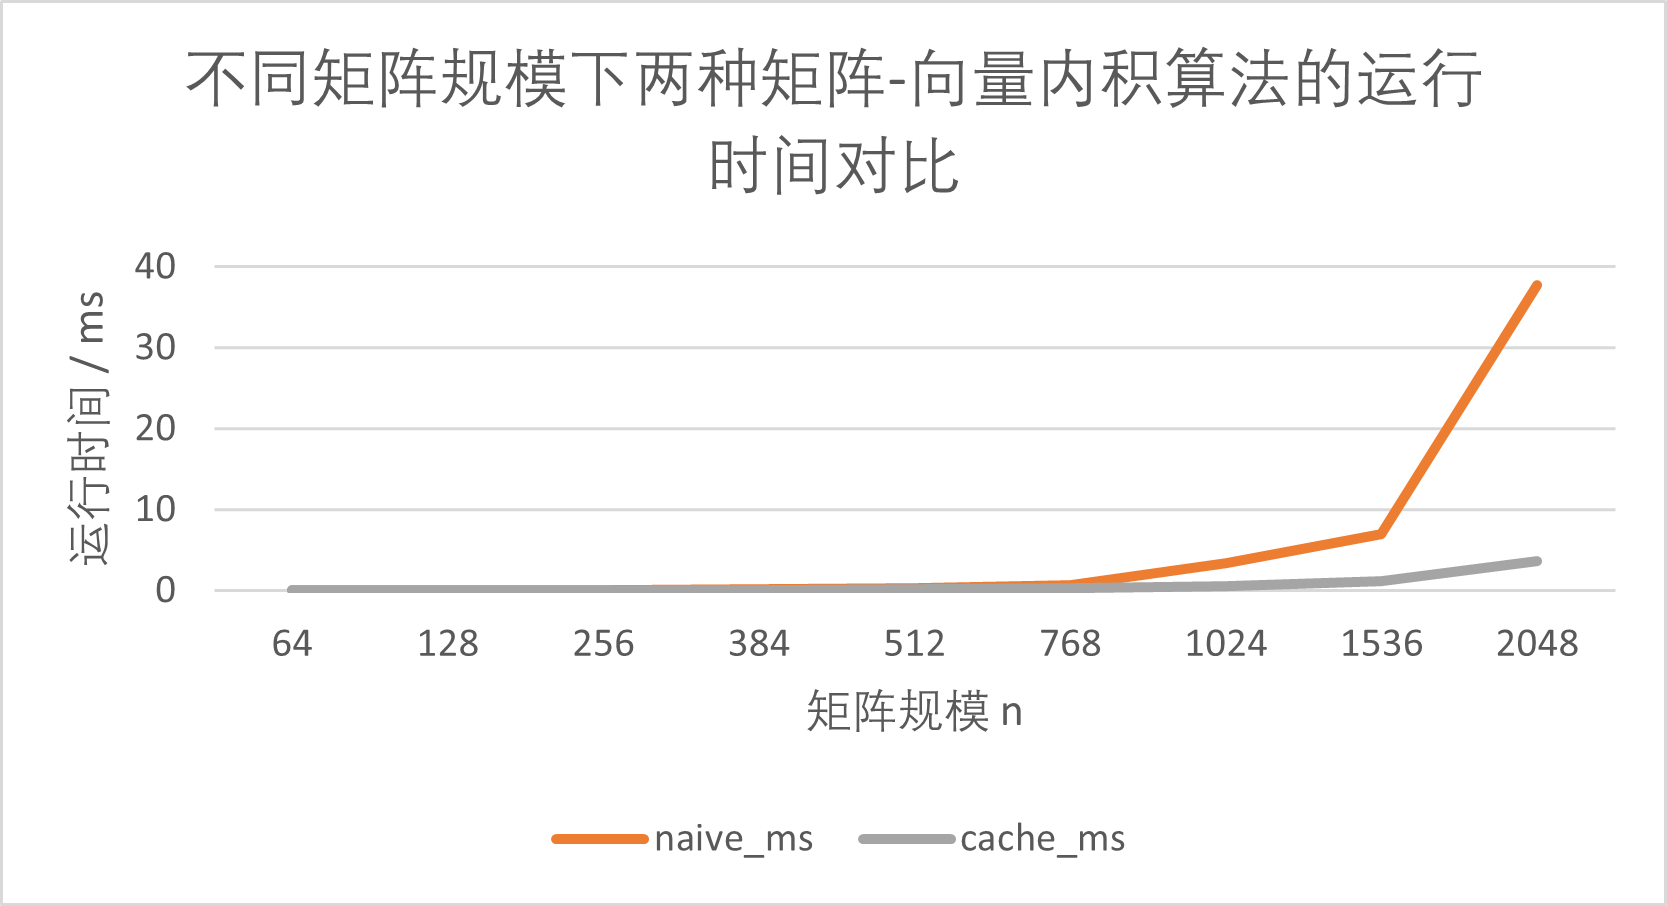
\includegraphics[width=0.92\textwidth]{fig/dot_basic_O2.png}
\caption{不同矩阵规模下平凡算法与 cache 优化算法的运行时间对比}
\label{fig:dot-basic}
\end{figure}

\subsection{结果分析}
从表~\ref{tab:dot-basic} 可以看出，在问题规模较小时，两种算法的时间差距不大；例如 $n=64$ 时，cache 优化版本甚至略慢于平凡算法。这说明当数据规模较小时，矩阵数据仍能较好地驻留在低层缓存中，单纯调整循环顺序所带来的收益尚不明显。

随着 $n$ 增大，cache 优化算法的优势迅速体现出来。$n=512$ 时加速比已经达到 2.21 倍；当 $n=1024$ 时加速比提升到 6.67 倍；到 $n=2048$ 时进一步达到 10.35 倍。这表明该实验的性能瓶颈主要不是乘加次数，而是访存模式。平凡算法按列访问矩阵，在行主存储布局下会频繁跨越不同 cache line，导致缓存利用率较低；而优化算法按行连续读取矩阵元素，能够显著改善空间局部性，因此在规模增大后表现出明显更高的吞吐能力。

结合本机 2.1 MB 的 L1 Cache、32.0 MB 的 L2 Cache 和 36.0 MB 的 L3 Cache 可以进一步理解这一现象：随着矩阵规模增大，数据逐渐超过低层缓存容量，访存模式对性能的影响被放大，因此两种算法之间的差距在大规模区间显著拉大。

\section{实验二：$n$ 个数求和}
\subsection{算法设计}
第二个实验要求计算长度为 $n$ 的数组元素之和。平凡算法使用单个累加器，从头到尾逐个执行 \texttt{sum += a[i]}。这种写法虽然最简单，但每一步运算都依赖上一步的结果，会形成较长的数据相关链，从而限制处理器流水线和超标量发射单元的并行能力。

优化算法采用两路链式累加的思路：使用两个独立的累加器分别处理不同位置的数组元素，最后再把两个部分和相加。这样可以将一条很长的依赖链拆分为两条较短且彼此独立的依赖链，从而更好地发挥处理器的指令级并行能力。该优化并未减少总加法次数，但改善了指令调度条件，因此有望提高执行效率。

\subsection{实验结果}
表~\ref{tab:sum-basic} 给出了在 \texttt{-O2} 编译下链式平凡算法和两路链式累加算法的测试结果。

\begin{table}[H]
\centering
\caption{$n$ 个数求和基础测试结果}
\label{tab:sum-basic}
\setlength{\tabcolsep}{4pt}
\footnotesize
\begin{tabularx}{\textwidth}{P{1.65cm}P{1.65cm}P{1.55cm}P{1.45cm}YY}
\toprule
$n$ & naive\_ms & dual\_ms & speedup & repeats\_naive & repeats\_dual \\
\midrule
1024     & 0.000875 & 0.000533 & 1.639727 & 390624 & 390624 \\
4096     & 0.004069 & 0.002179 & 1.867015 & 97656  & 195312 \\
16384    & 0.016338 & 0.007393 & 2.209832 & 24414  & 48828 \\
65536    & 0.059309 & 0.032988 & 1.797910 & 6102   & 6102 \\
262144   & 0.235940 & 0.125555 & 1.879175 & 1524   & 3048 \\
1048576  & 1.124038 & 0.594254 & 1.891511 & 190    & 380 \\
4194304  & 4.968629 & 3.002182 & 1.655006 & 94     & 94 \\
16777216 & 19.795482 & 19.021014 & 1.040716 & 11    & 22 \\
\bottomrule
\end{tabularx}
\end{table}

\begin{figure}[H]
\centering
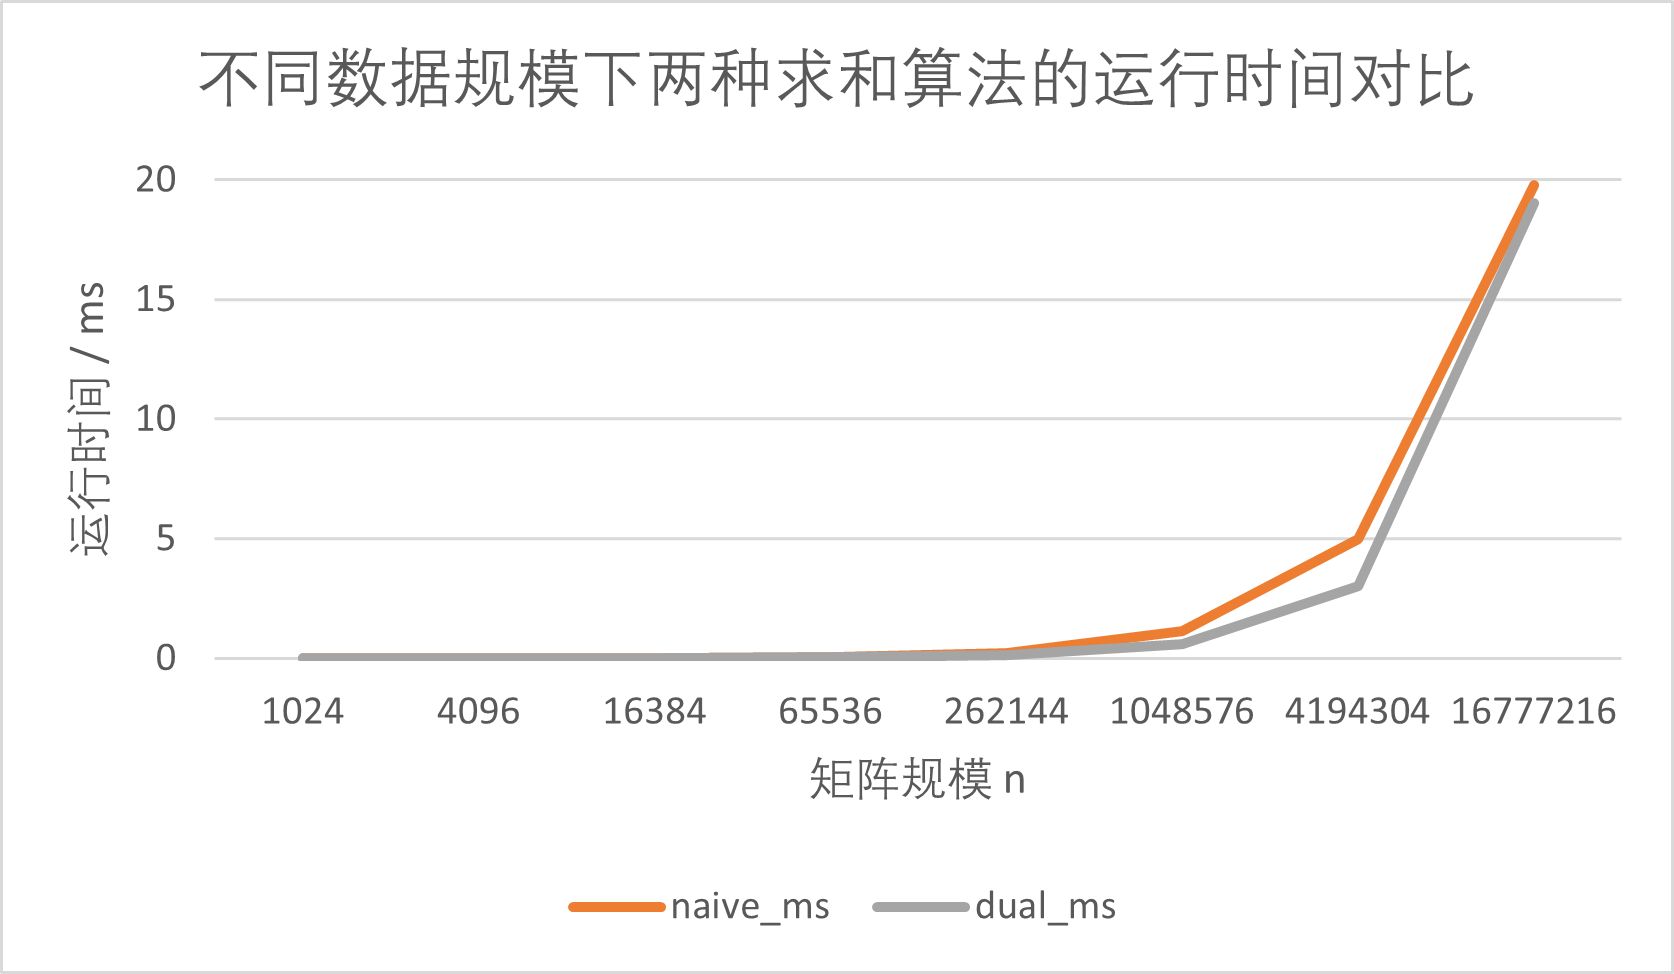
\includegraphics[width=0.92\textwidth]{fig/sum_basic_O2.png}
\caption{不同数据规模下链式累加与两路链式累加的运行时间对比}
\label{fig:sum-basic}
\end{figure}

\subsection{结果分析}
从表~\ref{tab:sum-basic} 可以看出，两路链式累加算法在大多数规模下都优于平凡算法。较为典型的是 $n=16384$ 时，加速比达到 2.21 倍；在 $n=262144$ 和 $n=1048576$ 时，加速比分别为 1.88 倍和 1.89 倍。说明把单累加器改为双累加器之后，确实能够减少指令之间的串行依赖，提高处理器的并行执行效率。

不过当规模继续增大到 $n=16777216$ 时，加速比下降到 1.04 倍，优化效果明显减弱。这说明在超大规模下，程序性能已不再主要受算术依赖限制，而更多受到内存访问带宽、缓存层次和总体数据搬移开销的影响。换言之，在问题规模较小时，超标量优化能够明显提升求和效率；而当数据规模巨大时，访存开销逐渐成为新的主要瓶颈，导致双链路累加相对平凡算法的优势被削弱。

\section{进阶要求一：循环展开与额外算法对比}
\subsection{实现方式说明}
在基础版本之外，当前代码已经额外实现了 \texttt{dot\_cache\_unroll4}、\texttt{sum\_dual\_unroll4} 和 \texttt{sum\_pairwise} 三个版本。其中，前两个版本直接对应课程所要求的“循环展开”方向：它们在保持算法主思路不变的前提下，通过一次循环处理多个元素来减少循环控制开销，并为编译器提供更多指令级并行空间。\texttt{sum\_pairwise} 则属于扩展性实现，用于观察树形归约结构在串行 CPU 上的实际表现。

当前压缩包中的 \texttt{code/results/dot\_advanced\_O2.csv} 和 \texttt{code/results/sum\_advanced\_O2.csv} 已经给出了这些版本在 \texttt{-O2} 下的测试结果，因此这一部分不需要再改 C 代码，只需要把结果整理进报告即可。

\subsection{矩阵内积循环展开结果}
表~\ref{tab:dot-unroll} 选取了四组代表性规模，对比 cache 优化版本与 4 路展开版本。

\begin{table}[H]
\centering
\caption{矩阵内积中循环展开的代表性结果（\texttt{-O2}）}
\label{tab:dot-unroll}
\setlength{\tabcolsep}{4pt}
\footnotesize
\begin{tabularx}{\textwidth}{P{1.25cm}P{1.85cm}P{2.2cm}P{1.75cm}P{1.95cm}}
\toprule
$n$ & cache\_ms & cache\_unroll4\_ms & speedup\_cache & speedup\_unroll4 \\
\midrule
256  & 0.031533 & 0.024789 & 1.927994 & 2.452498 \\
512  & 0.115108 & 0.098604 & 2.207516 & 2.577014 \\
1024 & 0.500330 & 0.489865 & 6.665738 & 6.808147 \\
2048 & 3.649994 & 3.443459 & 10.347132 & 10.967743 \\
\bottomrule
\end{tabularx}
\end{table}

从表~\ref{tab:dot-unroll} 可以看出，在矩阵内积实验中，循环展开总体上带来了进一步加速。特别是在 $n=256$、$512$ 和 $2048$ 时，\texttt{cache\_unroll4} 的时间都低于普通 \texttt{cache} 版本；在 $n=2048$ 时，展开后的总加速比从 10.35 倍提升到 10.97 倍。说明当访存模式已经被优化后，循环展开仍可以通过减少分支判断和归纳变量更新带来一定收益。不过这种收益小于“列访问改为行访问”本身所带来的收益，因此在本题中，\textbf{cache 局部性仍是第一主导因素，循环展开属于次一级优化}。

\subsection{$n$ 个数求和的展开与额外算法结果}
表~\ref{tab:sum-advanced} 选取了四组规模，对比 \texttt{dual}、\texttt{dual\_unroll4} 和 \texttt{pairwise} 三种扩展版本。

\begin{table}[H]
\centering
\caption{$n$ 个数求和进阶结果（\texttt{-O2}）}
\label{tab:sum-advanced}
\setlength{\tabcolsep}{3pt}
\footnotesize
\begin{tabularx}{\textwidth}{P{1.55cm}P{1.35cm}P{1.7cm}P{1.35cm}P{1.45cm}P{1.8cm}}
\toprule
$n$ & dual\_ms & dual\_unroll4\_ms & pairwise\_ms & speedup\_dual & speedup\_dual\_unroll4 \\
\midrule
16384    & 0.007393 & 0.004413 & 0.011743 & 2.209832 & 3.702346 \\
262144   & 0.125555 & 0.080771 & 0.511040 & 1.879175 & 2.921115 \\
1048576  & 0.594254 & 0.310325 & 2.339208 & 1.891511 & 3.622135 \\
16777216 & 19.021014 & 16.754614 & 59.875982 & 1.040716 & 1.181494 \\
\bottomrule
\end{tabularx}
\end{table}

这组结果显示，\texttt{dual\_unroll4} 的表现明显优于基础的 \texttt{dual} 版本。在 $n=16384$ 和 $n=1048576$ 时，展开后相对平凡算法的加速比分别达到 3.70 倍和 3.62 倍，显著高于双链路但未展开的版本。这说明在求和问题中，减少依赖链与减少循环控制开销能够形成叠加收益。相比之下，\texttt{pairwise} 版本只在很小规模时略有优势，随着规模增大很快落后于其他版本；例如在 $n=262144$ 时，其相对平凡算法的加速比已经下降到 0.46。这表明树形归约结构虽然在并行算法设计中较常见，但在当前串行实现里，多轮写回与额外的数据移动会抵消其理论优势。

\placeholderbox{进阶部分可补充图片：循环展开版本对比图}{建议后续从 \texttt{dot\_advanced\_O2.csv} 和 \texttt{sum\_advanced\_O2.csv} 各绘制 1 张图。\\
矩阵题建议画 \texttt{cache\_ms} 与 \texttt{cache\_unroll4\_ms}；\\
求和题建议画 \texttt{dual\_ms}、\texttt{dual\_unroll4\_ms}、\texttt{pairwise\_ms}。}

\section{进阶要求二：不同编译优化力度对比}
\subsection{实现与数据来源}
课程说明鼓励比较不同编译优化选项对性能的影响。对应地，当前代码包已经提供了 \texttt{run\_flags\_compare.bat}，并且你上传的结果目录中已经包含 \texttt{dot\_basic\_O0.csv}、\texttt{dot\_basic\_O2.csv}、\texttt{dot\_basic\_O3.csv} 以及求和实验的三组对应文件。因此，这一部分同样不需要再修改代码，只需继续补充图表或在需要时重新运行脚本复现实验即可。

\subsection{代表性结果}
为避免表格过大，这里只选取两个最能体现差异的代表性规模：矩阵内积取 $n=2048$，求和实验取 $n=1048576$。

\begin{table}[H]
\centering
\caption{不同编译优化等级下的代表性结果}
\label{tab:flags}
\setlength{\tabcolsep}{5pt}
\footnotesize
\begin{tabularx}{\textwidth}{Y P{1.75cm} P{1.75cm} P{1.75cm}}
\toprule
实验项目 & \texttt{-O0} & \texttt{-O2} & \texttt{-O3} \\
\midrule
矩阵内积 naive ($n=2048$) & 61.113700 & 37.766971 & 33.720876 \\
矩阵内积 cache ($n=2048$) & 9.084500 & 3.649994 & 1.250651 \\
求和 naive ($n=1048576$) & 3.534792 & 1.124038 & 0.422897 \\
求和 dual ($n=1048576$) & 2.041303 & 0.594254 & 0.211015 \\
\bottomrule
\end{tabularx}
\end{table}

从表~\ref{tab:flags} 可以看出，编译器优化等级对两类程序均有显著影响。对于矩阵内积，\texttt{-O3} 相比 \texttt{-O2} 仍能继续降低运行时间，尤其是 cache 优化版本从 3.65 ms 进一步下降到 1.25 ms，说明在访存模式已经较优的前提下，更高的编译器优化仍可能通过更积极的循环与指令调度挖掘额外性能。对于求和实验，\texttt{-O0} 与 \texttt{-O2}/\texttt{-O3} 的差距同样明显，说明寄存器分配、指令调度和循环优化对简单归约程序也具有重要影响。整体来看，\texttt{-O2} 适合作为基础实验的默认编译选项，而 \texttt{-O3} 则更适合在进阶部分考察“编译器还能帮我们做多少事”。

\placeholderbox{进阶部分可补充图片：编译优化等级对比图}{建议后续至少补 1 张图。\\
做法：从三组 O0/O2/O3 的 CSV 中选取同一列数据，画成柱状图或折线图。\\
矩阵题可画 \texttt{cache\_ms} 对比，求和题可画 \texttt{dual\_ms} 或 \texttt{dual\_unroll4\_ms} 对比。}

\section{进阶要求三：Godbolt 汇编分析（待补截图）}
当前代码中的 \texttt{sum\_naive}、\texttt{sum\_dual\_unroll4}、\texttt{dot\_cache} 和 \texttt{dot\_cache\_unroll4} 都适合拿到 Godbolt 中做汇编观察。建议优先比较以下两组：
\begin{enumerate}
    \item \texttt{sum\_naive} 与 \texttt{sum\_dual\_unroll4}：观察寄存器数量、循环体中加法指令的组织方式，以及是否形成多条独立累加链；
    \item \texttt{dot\_cache} 与 \texttt{dot\_cache\_unroll4}：观察循环体是否变长、是否减少了循环控制相关指令。
\end{enumerate}

这一部分需要你自己到 \texttt{https://godbolt.org} 上截图，因此报告中只先留出位置。截图补上以后，本节可以直接增加两段文字：第一段解释“展开后汇编为何更有利于流水线发射”，第二段解释“编译器在 \texttt{-O3} 下是否自动做了部分展开或向量化前处理”。

\placeholderbox{Godbolt 汇编截图占位图}{此处需你自行补图。建议至少放 2 张截图：\\
(1) \texttt{sum\_naive} vs \texttt{sum\_dual\_unroll4}；\\
(2) \texttt{dot\_cache} vs \texttt{dot\_cache\_unroll4}。}

\section{进阶要求四：VTune / perf profiling（可选待补）}
从课程要求看，profiling 属于推荐但非强制完成项。考虑到你当前主要在 Windows 原生环境下完成实验，这一部分更适合作为最后补充：如果你后续安装 VTune，可以优先对矩阵内积的 \texttt{naive} 与 \texttt{cache} 两个版本做热点与 memory bound 分析；如果后续切换到 WSL/Linux，再尝试使用 \texttt{perf stat} 或 \texttt{perf record} 统计 cache miss、instructions 和 cycles 等指标。

本节在当前版本中只保留分析框架，不硬填虚假数据。后续真正补 profiling 时，建议围绕两个问题展开：一是“为什么矩阵内积的 cache 版在大规模时优势迅速扩大”；二是“为什么求和实验中 \texttt{dual\_unroll4} 的优势会在超大规模时减弱”。这样写出来的 profiling 部分才真正服务于性能分析，而不是堆砌工具截图。

\placeholderbox{VTune / perf 结果占位图}{此处需你自行补图。可以放热点视图、memory bound 视图，或 \texttt{perf stat} 的关键计数结果。}

\section{后续完成顺序说明}
如果按照“工作量最小、收益最高”的顺序继续完成剩余进阶要求，建议按以下流程进行：
\begin{enumerate}
    \item \textbf{先直接写进报告的内容}：本模板中的“循环展开”和“不同编译优化力度对比”已经可以直接使用，因为相应数据已在你上传的结果目录中存在；
    \item \textbf{接着补 2 张进阶图}：一张来自 \texttt{dot\_advanced\_O2.csv}，一张来自 \texttt{sum\_advanced\_O2.csv}；这一步只需要画图，不需要改代码；
    \item \textbf{再补 Godbolt 截图}：这是当前最容易完成、最适合展示“你理解了代码为什么变快”的部分；
    \item \textbf{最后再考虑 VTune / perf}：如果时间不够，可以把本节保留为占位并在报告中明确说明“此项为可选扩展，后续将结合 Linux/VTune 环境继续完成”。
\end{enumerate}

\section{结论}
本次实验围绕 cache 与超标量两类典型体系结构特性，对两个简单但具有代表性的计算问题进行了实现与测试。对于矩阵每列与向量内积问题，平凡算法和 cache 优化算法的主要差异体现在访存顺序上。实验结果表明，随着矩阵规模增大，按行连续访问的优化版本能够显著降低缓存失效带来的性能损失，在大规模下取得超过 10 倍的加速效果。对于 $n$ 个数求和问题，两路链式累加通过缩短单条依赖链、提高指令级并行性，在多数规模下都优于逐个累加的平凡算法，但其优势会在超大规模数据下因访存带宽限制而减弱。

在进阶部分中，循环展开版本与编译器优化等级对比已经通过现有代码和结果文件得到了初步验证：矩阵内积中的 \texttt{cache\_unroll4} 相比普通 \texttt{cache} 版本仍有一定提升，求和实验中的 \texttt{dual\_unroll4} 则比 \texttt{dual} 版本表现更稳定；同时，\texttt{-O3} 相比 \texttt{-O2} 仍能进一步挖掘部分性能。剩余尚未补齐的主要是 Godbolt 和 VTune/perf 的截图与说明，这些部分不涉及重复写代码，只需要按当前模板继续补图与补充分析即可。

\end{document}
